\documentclass{ctexart}
\usepackage{amsmath,amsthm,amssymb,stmaryrd}
\usepackage{fullpage}
\usepackage{graphicx}
\usepackage{algorithm,algorithmic}
\usepackage[bookmarksnumbered,bookmarksopen,colorlinks=true,citecolor=red,anchorcolor=blue,linkcolor=blue,CJKbookmarks=true]{hyperref}

\usepackage{tikz}
\tikzset{eaxis/.style={->,>=stealth}}
\tikzset{elegant/.style={smooth,thick,samples=200,black}}

\usepackage{bm}
\usepackage{enumitem}
\setenumerate[1]{itemsep=0pt,partopsep=0pt,parsep=\parskip,topsep=0pt}
\setitemize[1]{itemsep=0pt,partopsep=0pt,parsep=\parskip,topsep=0pt}
\setdescription{itemsep=0pt,partopsep=0pt,parsep=\parskip,topsep=0pt}

\usepackage{fontspec} 
\setCJKmainfont[BoldFont=FZHei-B01,ItalicFont=FZHei-B01]{方正苏新诗柳楷简体-yolan}

\theoremstyle{definition}
\newtheorem{thm}{定理}
\newtheorem{prop}{命题}
\newtheorem{lem}{引理}
\newtheorem{cor}{推论}
\newtheorem{defn}{定义}
\newtheorem{exam}{例}
\newtheorem*{exc}{习题}
\newtheorem*{ans}{解答}
\newtheorem*{rmk}{注}
\renewcommand{\proofname}{证明}
\renewcommand{\qedsymbol}{M.X.}

\DeclareMathOperator*{\argmin}{argmin}
\DeclareMathOperator*{\argmax}{argmax}

\def \zerov {\bm{0}}
\def \av {\bm{a}}
\def \bv {\bm{b}}
\def \ev {\bm{e}}
\def \sv {\bm{s}}
\def \uv {\bm{u}}
\def \wv {\bm{w}}
\def \Av {\bm{A}}
\def \Gv {\bm{G}}
\def \Iv {\bm{I}}
\def \Uv {\bm{U}}
\def \lambdav {\bm{\lambda}}
\def \Rbb {\mathbb{R}}

\def \Oca\alpha {\mathcal{O}}

\def \st {\mathrm{s.t.}}
\def \ow {\mathrm{o.w.}}
\def \diff {\mathrm{d}}

\begin{document}
\title{}
\date{}
\maketitle

\thispagestyle{empty}

\begin{figure}[ht]
  \centering
  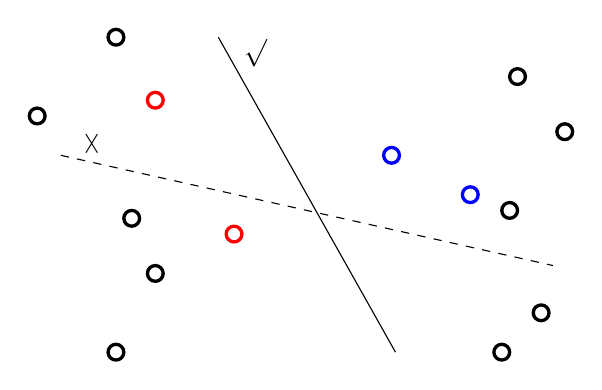
\begin{tikzpicture}[scale=1.0]

    %\draw[loosely dotted] (2.5,0) ellipse (2 and 3);
    %\draw[loosely dotted] (-2.5,0) ellipse (2 and 3);

    
    \draw[very thick] (-3.5,1) circle (0.1);
    \draw[very thick] (-2.5,2) circle (0.1);
    \draw[red,very thick] (-2,1.2) circle (0.1);

    \draw[very thick] (-2.3,-0.3) circle (0.1);
    \draw[very thick] (-2.5,-2) circle (0.1);
    \draw[very thick] (-2,-1) circle (0.1);
    \draw[red,very thick] (-1,-0.5) circle (0.1);

    \draw[very thick] (2.6,1.5) circle (0.1);
    \draw[very thick] (3.2,0.8) circle (0.1);

    \draw[blue,very thick] (1,0.5) circle (0.1);
    \draw[blue,very thick] (2,0) circle (0.1);
    \draw[very thick] (2.5,-0.2) circle (0.1);

    \draw[very thick] (2.9,-1.5) circle (0.1);
    \draw[very thick] (2.4,-2) circle (0.1);
    
    %\draw[loosely dashed] (-1,-0.5) -- (1.14, 0.64);
    %\draw[loosely dashed] (-2.3,-0.3) -- (2.64, -0.06);

    \draw (-1.2,2) -- (1.05, -2);
    \path (-1,1.8) node[draw=none,right] () {$\surd$};

    \draw[dashed] (-3.2,0.5) -- (3.05, -0.9);
    \path (-2.8,0.4) node[draw=none,above] () {$\vartimes$};

    %\draw[very thick] (-0.05,2.8989) -- (0.37, -2.8644);

  \end{tikzpicture}
  \caption{}
\end{figure}


\end{document}